
\documentclass{article}

%% Packages for French writing
\usepackage[french]{babel}
\usepackage[utf8]{inputenc}
\usepackage[T1]{fontenc}
\usepackage{layout}

%% Packages for Math symbols
\usepackage[fleqn]{amsmath}
\usepackage{amssymb}
\usepackage{mathrsfs}

%% Packages for figures insertion
\usepackage{graphicx}
\usepackage{wrapfig}
\usepackage{framed}
\usepackage{float}

%% Package for document margin editing
\usepackage[top=2cm, bottom=2cm, left=2cm, right=2cm]{geometry}

%% Package for source code insertion
\usepackage{listings}
\usepackage{xcolor}
\definecolor{grey}{rgb}{0.97, 0.97, 0.97}
\definecolor{darkred}{rgb}{0.42, 0, 0}
\definecolor{darkblue}{rgb}{0, 0, 0.42}
\definecolor{darkgrey}{rgb}{0.22, 0.22, 0.82}
\definecolor{green}{HTML}{088A08}
\lstset{
  basicstyle=\small\sffamily\footnotesize,
  captionpos=b,
  numbers=left,
  numberstyle=\tiny,
  tabsize=4,
  frame=trBL,
  backgroundcolor=\color{grey},
  commentstyle=\color{green},
  keywordstyle=\color{darkblue}\bf,
  identifierstyle=\color{darkgrey},
  stringstyle=\color{darkred}
}

\setlength\parindent{0pt}
\setlength\parskip{3pt}
\title{Rapport de projet VLSI}
\author{Nicolas Phan, Kevin Mambu}
\date{pour le 26 Janvier 2018}
\begin{document}
\pagestyle{headings}
\maketitle
\tableofcontents
\newpage

%==================================================================================================
%=========================  Introduction  =========================================================
%==================================================================================================
\section{Introduction}

%----------------- Objectif -----------------------------------------------------------------------
\subsection{Objectif}

Le but de notre projet est de concevoir un processeur ARM, c'est à dire un processeur conforme
à l'architecture décrite dans la documentation ARM donnée en cahier des charges.

%----------------- Processus de developpement -----------------------------------------------------
\subsection{Processus de développement}

La conception de ce processeur se fera en cinq grandes étapes :

\begin{figure}[H]
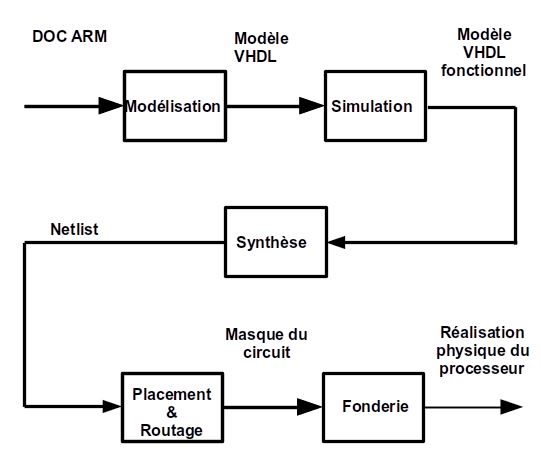
\includegraphics[width=0.75\textwidth]{pics/conception1.png}
\centering
\caption{Schema-bloc des étapes de conception du processeur}
\label{conception}
\end{figure}

\begin{enumerate}
\item \textbf{Modélisation}  : Cela consiste en la description d'un modèle du processeur,
                      la description peut avoir différents niveaux d'abstraction
                      du plus abstrait (description du comportement du circuit seulement)
                      au plus concret (schema des portes logiques du circuit)
                      \textit{Nous utiliserons le langage VHDL pour décrire notre modèle de processeur}
\item \textbf{Simulation}    : Il s'agit de vérifier par la simulation que notre modèle est fonctionnel.
                      \textit{Nous utiliserons le simulateur ghdl ainsi que des bancs de tests VHDL
                      et une plateforme de simulation d'exécution de programmes ASM et C pour cela.}
\item \textbf{Synthèse} : Cette étape consiste à passer de notre modèle VHDL fonctionnel à une description
                          concrète du circuit (en portes logiques, transistors), autrement dit une netlist.
                          \textit{Nous utiliserons les outils vasy, bool et boog ici.}
\item \textbf{Placement, Routage} : Dans cette étape, nous passons de la netlist à un
                          dessin du masque de notre processeur, prêt à être envoyé en fonderie.
                          \textit{Nous utiliserons les outils druc, cougar, lvx, tas et s2r pour cela.}
\item \textbf{Fonderie} :          Cette étape est réalisée par un fondeur tiers.
\end{enumerate}

La Figure \ref{outils} résume le flot de travail et les outils utilisés pour les étapes de Syntèse,
Placement et Routage.

\begin{figure}[H]
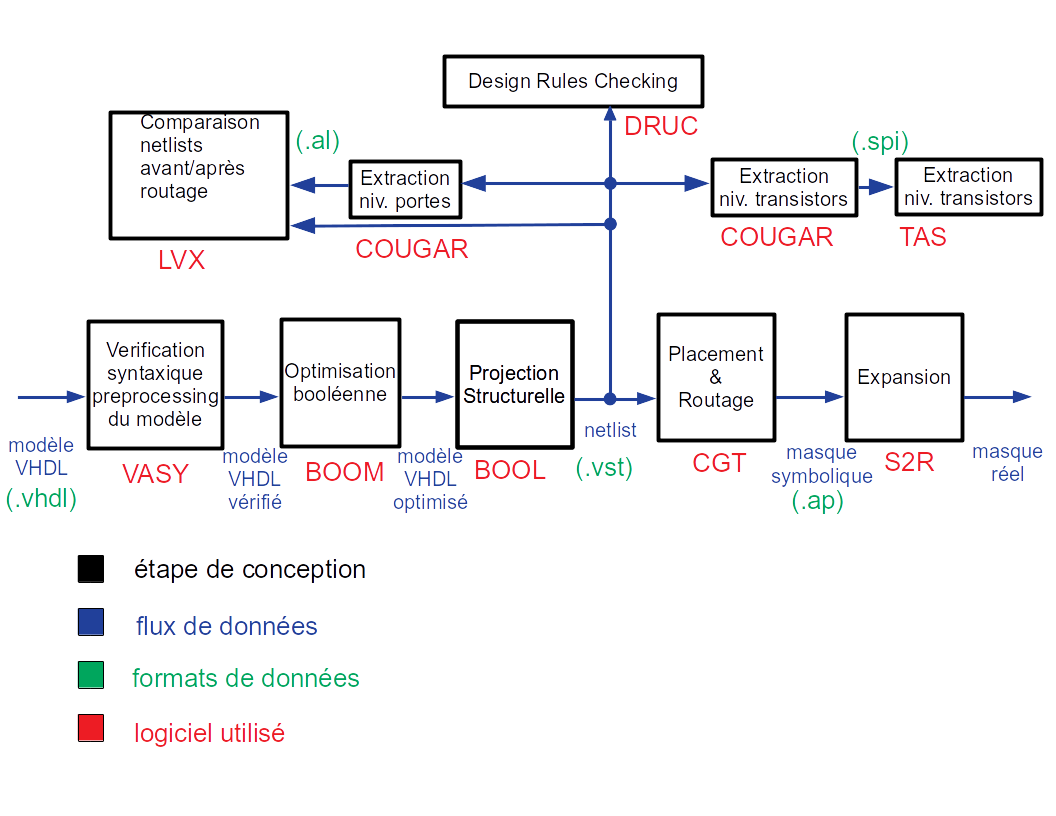
\includegraphics[width=0.75\textwidth]{pics/conception2.png}
\centering
\caption{Outils utilisés pour la réalisation du processeur}
\label{outils}
\end{figure}

%==================================================================================================
%=========================  Modelisation  =========================================================
%==================================================================================================
\section{Modélisation}

%==================== Design general du processeur ================================================
\subsection{Design général du processeur}

Le processeur que nous voulons réaliser doit pouvoir exécuter toutes les instruction du jeu ARM
mais nous nous concentrerons sur instructions de data processing (regops),
les instructions de branchement (branch), les transferts mémoires simples (trans) et multiples (mtrans).

Le processeur doit pouvoir exécuter ces instructions le plus rapidement possible, et pour arriver à des
performances satisfaisantes nous choisissons de concevoir un processeur pipeliné (pipeliné asynchrone).

Dès lors que nous choisissons une architecture pipelinée, une première étape est d'énumérer l'ensemble
des traitement devant être effectués par le processeur pour pouvoir exécuter le jeu d'instructions,
et la répartition de ces traitement entre les différents étages, ceci est détaillé en Figure \ref{etages}.

\begin{figure}[H]
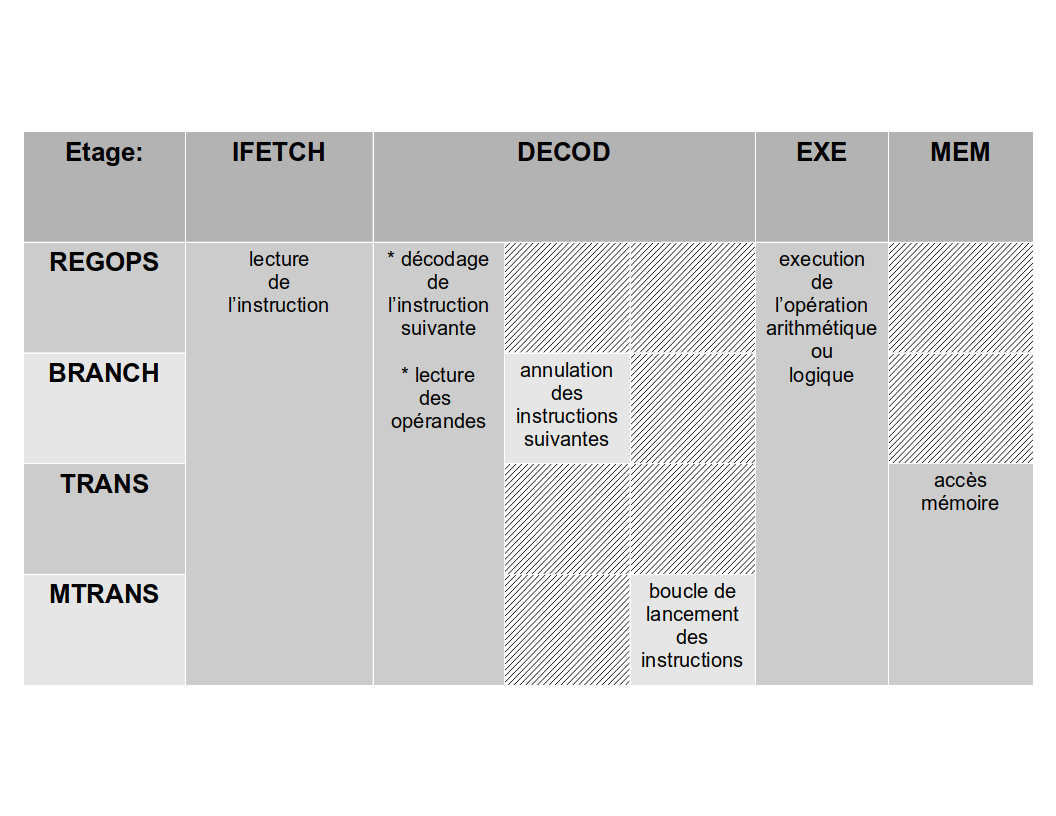
\includegraphics[width=0.75\textwidth]{pics/blank.png}
\centering
\caption{Découpage en étages du processeur}
\label{etages}
\end{figure}

Nous allons voir l'implémentation de l'étage EXEC, puis de DECOD.

%==================== Modelisation de l'etage EXE =================================================
\section{Modélisation de l'étage EXE}

\par
C'est à l'étage EXE que se feront les opérations de calcul lors de l'exécution d'instructions,
cela comprend les calculs classiques des instructions de data processing mais aussi le calcul de
l'adresse destination lors d'un branchement ou d'un accès mémoire.
Pour concevoir cet étage, nous devons nous demander quels sont tous les calculs possibles
que l'étage devra pouvoir réaliser.

\par
Les différents types d'instructions que nous avons sont les regops, les branch, les trans et mtrans.
Or les branch, trans et mtrans n'ont besoin d'effectuer que des additions (pour le calcul d'adresses
mémoire) et les regops contiennent des instructions d'addition, donc si l'étage EXE peut effectuer
les calculs nécéssaires aux regops, a fortiori il couvre aussi les branch et transferts mémoire.
Cela réduit le problème au cas des regops.

\par
Il faut lister l'ensemble des calculs que EXE devra effectuer et les réécrire
de manière standardisée pour les décomposer en un sous-ensemble d'opérations élémentaires.
Cela nous permettra de trouver une implémentation de EXE réduisant au maximum le matériel nécéssaire.

\begin{table}[H]
\centering
\begingroup
\setlength{\tabcolsep}{5pt}
\renewcommand{\arraystretch}{1.1}
\begin{tabular}{ | c | l | l | }
\hline
Instruction & Calcul demandé & Calcul standardisé  \\
\hline
\tt{AND}      & \tt{ op1 AND op2 }                 & \tt{ op1 AND op2 } \\
\hline
\tt{EOR}      & \tt{ op1 XOR op2 }                 & \tt{ op1 XOR op2 } \\
\hline
\tt{SUB}      & \tt{ op1 - op2 }                   & \tt{ op1 + $\overline{\tt{op2}}$ + 1 } \\
\hline
\tt{RSB}      & \tt{ op2 - op1 }                   & \tt{ $\overline{\tt{op1}}$ + op2 + 1} \\
\hline
\tt{ADD}      & \tt{ op1 + op2 }                   & \tt{ op1 + op2 } \\
\hline
\tt{ADC}      & \tt{ op1 + op2 + c }               & \tt{ op1 + op2 + c} \\
\hline
\tt{SBC}      & \tt{ op1 - op2 + c - 1 }           & \tt{ op1 + $\overline{\tt{op2}}$ + c} \\
\hline
\tt{RSC}      & \tt{ op2 - op1 + c - 1 }           & \tt{ $\overline{\tt{op1}}$ + op2 + c} \\
\hline
\tt{TST}      & \tt{ op1 AND op2 }                 & \tt{ op1 AND op2 } \\
\hline
\tt{TEQ}      & \tt{ op1 XOR op2 }                 & \tt{ op1 XOR op2 } \\
\hline
\tt{CMP}      & \tt{ op1 SUB op2 }                 & \tt{ op1 + $\overline{\tt{op2}}$ + 1 } \\
\hline
\tt{CMN}      & \tt{ op1 ADD op2 }                 & \tt{ op1 + op2 } \\
\hline
\tt{ORR}      & \tt{ op1 OR op2 }                  & \tt{ op1 OR op2 } \\
\hline
\tt{MOR}      & \tt{ op2 }                         & \tt{ 0 + op2 } \\
\hline
\tt{BIC}      & \tt{ op1 AND NOT op2 }             & \tt{ op1 AND $\overline{\tt{op2}}$ } \\
\hline
\tt{MVN}      & \tt{ NOT op2 }                     & \tt{ 0 + $\overline{\tt{op2}}$ } \\
\hline
\end{tabular}
\endgroup
\caption{Standardisation des calculs demandés par les regops}
\label{standard}
\end{table}

On peut voir sur la Table \ref{standard} que l'ensemble des calculs demandés se décompose
en opérations élémentaires suivantes :
\begin{enumerate}
  \item ADD, AND, OR, XOR
  \item Inversion des entrées au préalable
  \item Ajout d'un 1 pour l'addition (retenue en entrée)

De plus, le jeu d'instruction ARM spécife que l'opérande 1 peut subir un décalage
parmi 5 types (lsl, lsr, asr, ror, rrx) et qu'à chaque opération, les flags de sortie
doivent être calculés, on a donc en plus :
  \item Décalage de l'opérande 2
  \item Calcul des flags de sortie
\end{enumerate}

Avec ces 5 éléments, nous aboutissons au schema Figure \ref{exe_part} pour EXE.

\begin{figure}[H]
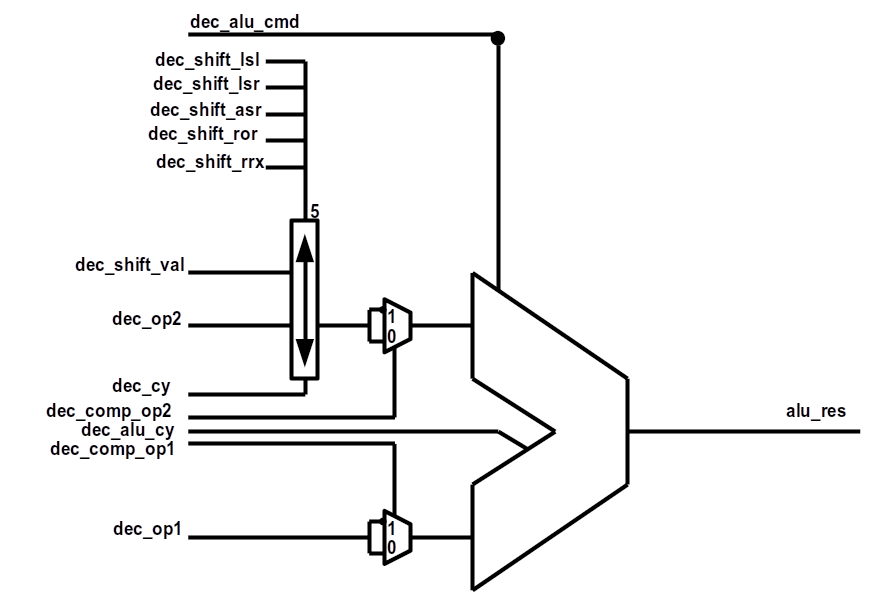
\includegraphics[width=0.75\textwidth]{pics/exe_part.png}
\centering
\caption{Schema partiel de l'étage EXE}
\label{exe_part}
\end{figure}

\subsection{Modélisation de l'ALU}

L'ALU doit pouvoir effectuer les opérations ADD, AND, OR et XOR sur deux entrées de 32bits,
et pour l'addition elle doit pouvoir prendre en compte une retenue en entrée et en sortie.

Notre implémentation est celle en Figure \ref{alu} : L'ALU effectue de toutes manières les
4 opérations sur ses entrées, mais ne prend que le résultat de l'opération qui nous intéresse.

Pour le calcul des flags, le bloc "=0" effectue un simple AND entre tous les bits du résultat,
le bloc "<0" vérifie si le MSB est égal à 1, on remarque que par la manière dont est construit
le système de nombres signés, la condition "<0" est très simple à vérifier. Puis pour le bloc "overflow",
on considère que les mots sont signés et il y a overflow si les deux opérandes sont de même signe et que
le résultat de l'addition est de signe différent.

\begin{figure}[H]
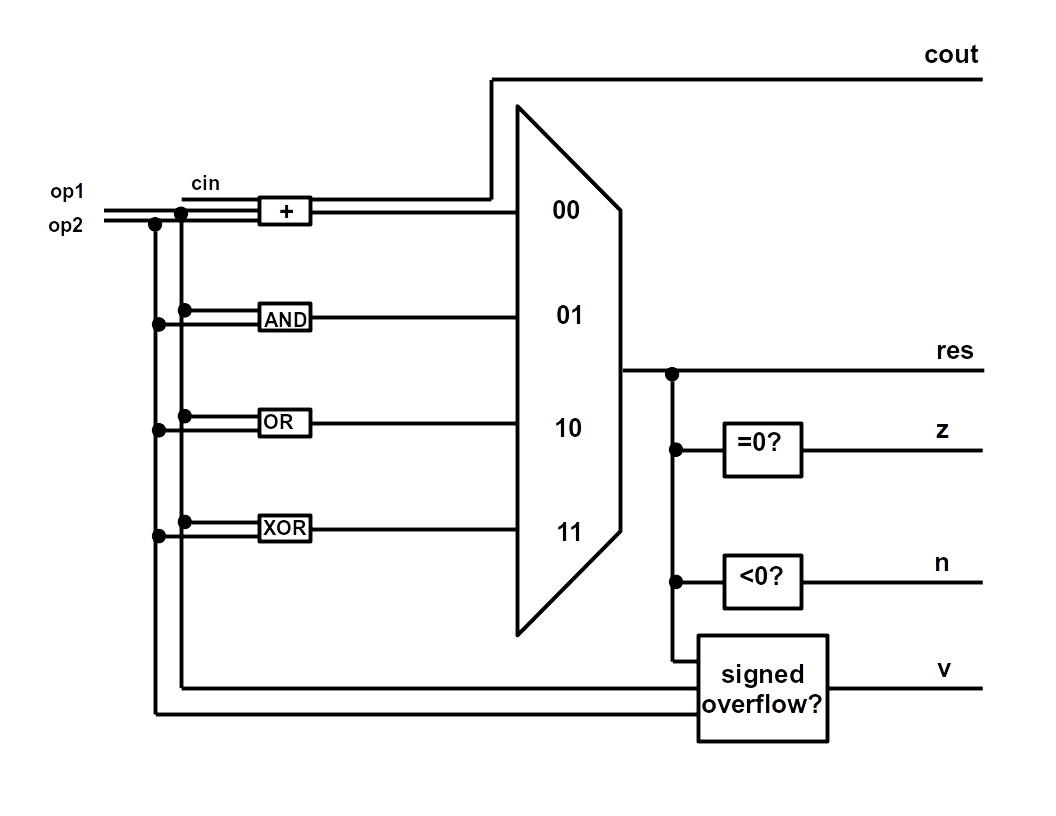
\includegraphics[width=0.75\textwidth]{pics/alu.png}
\centering
\caption{Schema de l'ALU}
\label{alu}
\end{figure}

\subsection{Modélisation du Shifter}

Tout comme l'ALU peut effectuer différentes opérations, le shifter peut effectuer différents
types de décalages (LSL, LSR, ASR, ROR, RRX) donc de la même manière, notre implémentation
du shifter en Figure \ref{shifter} effectue tous les types de décalages possibles et choisit
le résultat qui nous intéresse.

\begin{figure}[H]
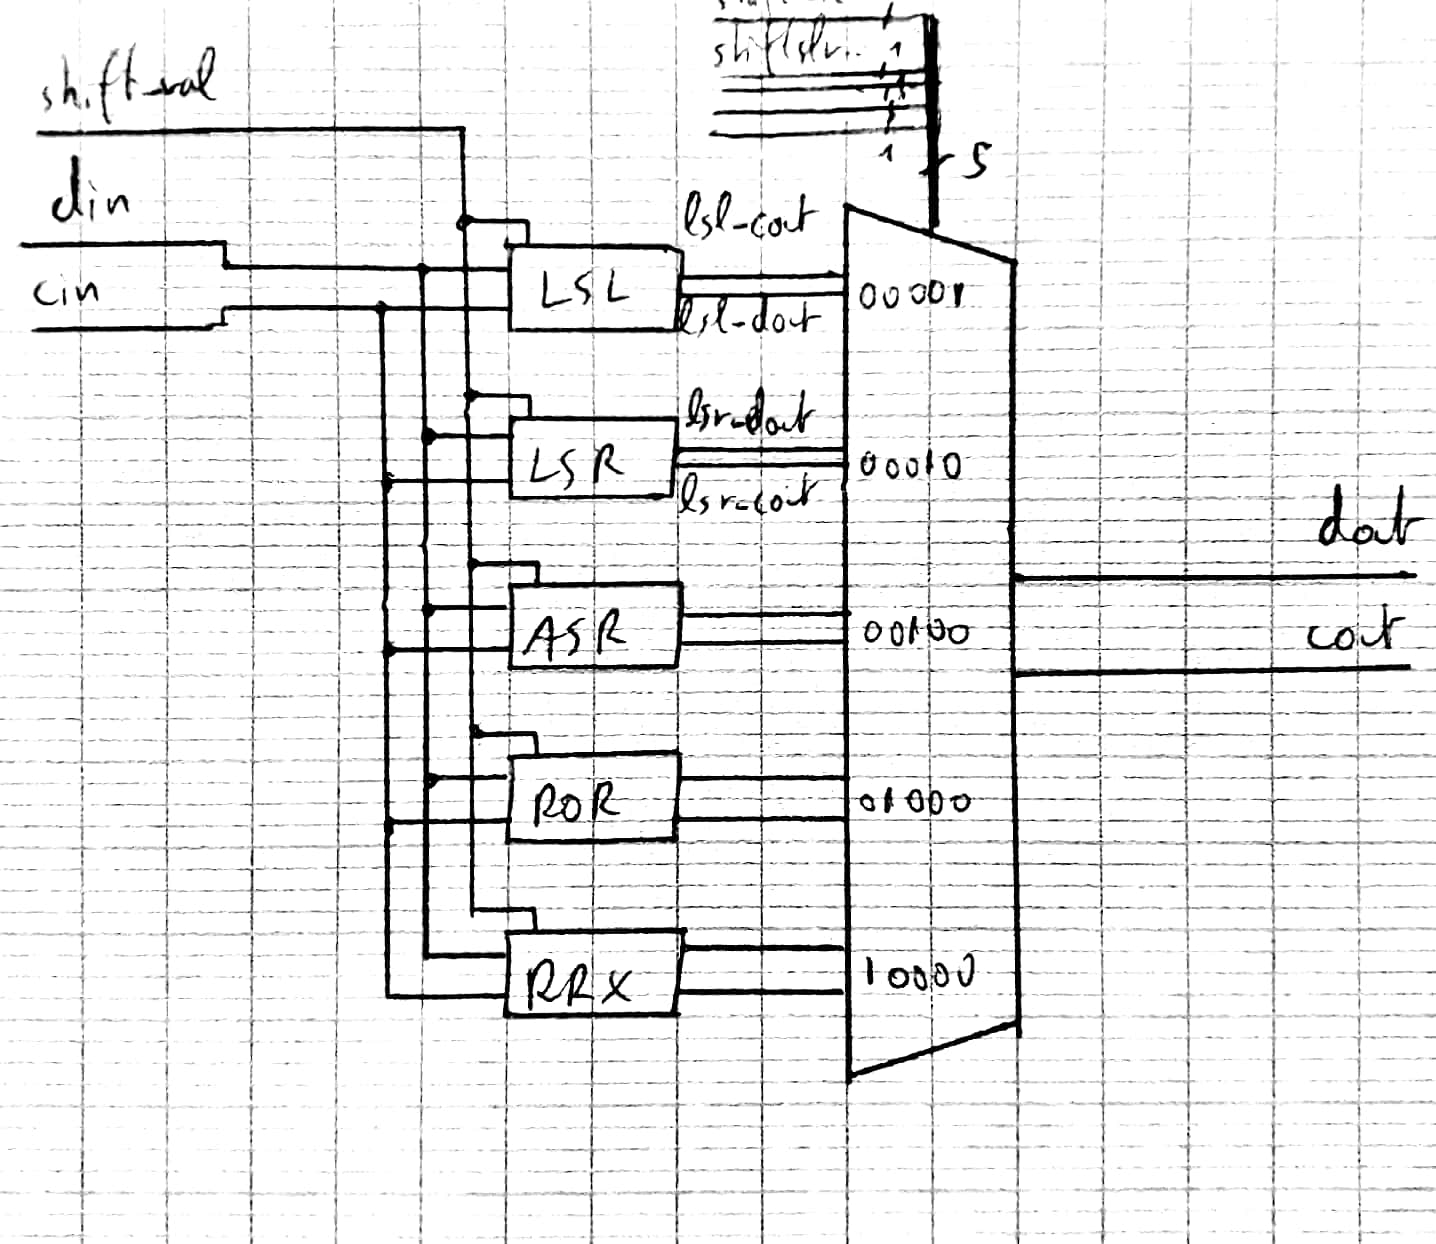
\includegraphics[width=0.75\textwidth]{pics/shifter.png}
\centering
\caption{Schema du Shifter}
\label{shifter}
\end{figure}

Ensuite pour réaliser l'opération LSL, en Figure \ref{shifter_lsl},
on observe chaque bit du \texttt{shift\_value} :
si le bit $n$ est à \texttt{1}, alors l'opérande subit un décalage de $2^n$.
Le décalage total subi par l'opérande source est donc de :

\begin{eqnarray*}
  \sum_{\substack{k \in [[0, 4]] \\ \texttt{shift\_value(k)} = 1}} 2^k &= \texttt{shift\_value}
\end{eqnarray*}

La même logique est utilisée pour implémenter les autres types de décalages.

\begin{figure}[H]
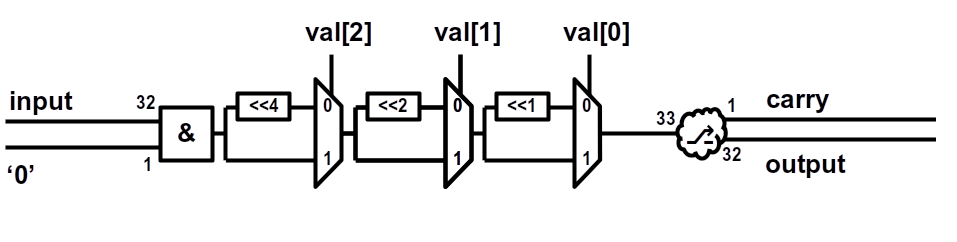
\includegraphics[width=0.75\textwidth]{pics/shifter_lsl.png}
\centering
\caption{Schema de la partie LSL du Shifter}
\label{shifter_lsl}
\end{figure}



\subsection{Ajouts sur EXE}

\textbf{Le flag C}

D'après la doc ARM, le flag C en sortie d'une opération peut être la retenue en sortie d'addition
pour les opérations arithmétiques ou en sortie de shift pour les opérations logiques.
Pour savoir si l'opération en cours est arithmérique ou logique, il suffit de voir si
l'ALU réalise une addition ou autre chose.

\textbf{La pre/post indexation}

Lors d'un accès mémoire, le jeu ARM offre la possibilité de choisisr si l'adresse prise en compte
pour un accès mémoire est l'adresse \texttt{base} ou l'adresse \texttt{base + offset}.
Dans EXE, cela équivaut à choisir entre l'opérande 2 et le résultat en sortie d'ALU,
cela mène au schema en Figure \ref{exe}.

\begin{figure}[H]
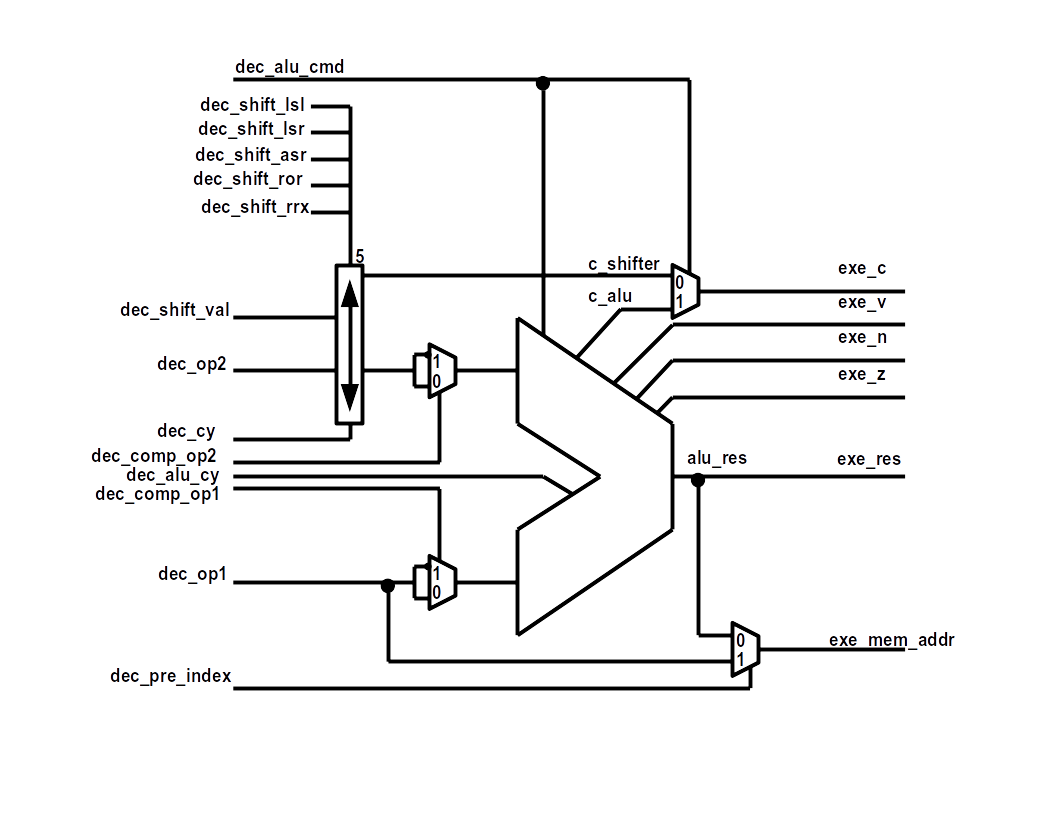
\includegraphics[width=0.75\textwidth]{pics/exe.png}
\centering
\caption{Schema amélioré de EXE}
\label{exe}
\end{figure}

%==================== Modelisation de l'etage DEC =================================================
\section{Modélisation de l'étage DECOD}

Pour chaque instruction, hormis quelques spécificités dues aux branchements
et transferts multiples, DECOD doit faire 7 choses :
\begin{enumerate}
  \item Envoyer l'adresse de l'instruction (valeur de PC) vers IFC.
  \item Récupérer l'instruction de IFC.
  \item Décoder l'instruction (quelle opération effectuer, quelles opérandes utiliser)
  \item Vérifier si la condition d'exécution est remplie (exécution conditionnelle)
  \item Lire dans le banc de registres les opérandes à utiliser.
  \item Envoyer les opérandes lues et le type d'opération à effectuer vers EXE.
  \item Passer à l'instruction suivante (incrémenter PC)
\end{enumerate}

Dans un premier temps, nous modéliserons le comportement général de DECOD,
puis nous apporterons des améliorations au fur et à mesure pour implémenter les branchements,
les branchements avec link puis les transferts multiples. Nous avons donc choisi une approche
"instruction par instruction" pour la modélisation de DECOD.

Le premier type d'instruction à implémenter sont les data processing instructions (regops),
elles ne font rien de spécial
dans DECOD donc il est approprié de commencer par elles.
Dans DECOD nous placerons le banc de registres (REG), nous verrons donc une par une les choses
à implémenter dans DECOD et dans REG.

\subsection{Envoi du PC vers IFC}

Nous plaçons dans REG la sortie \texttt{reg\_pc} qui donne à DEC la valeur de PC à chaque instant,
puis DEC transmet cette valeur à IFC sur la sortie \texttt{dec\_pc} via une FIFO (dec2if).

\subsection{Récupération de l'instruction depuis IFC}

Il y a encore communication entre deux étages, donc nous avons encore une FIFO (if2dec)
mais comme la convention veut que la FIFO soit à l'étage émetteur, elle sera dans IFC,
donc dans DEC nous récupérons simplement l'instruction via une entrée \texttt{if\_ir[32bits]}.

\subsection{Décodage de l'instruction}

\subsubsection{Decodage du type d'instruction}

Il s'agit ici de lire, à partir des 32 bits de \texttt{if\_ir}, quelle opération
doit être effectuée et sur quelles opérandes.

La première chose à décoder est le type d'instruction. Selon le détail du format des
instructions dans la documentation ARM, en ne considérant que les instructions :
\begin{enumerate}
  \item Data processing
  \item Multiply
  \item Single Data Swap
  \item Single Data Transfert
  \item Block Data Transfert
  \item Branch
\end{enumerate}

Le premier critère est que les bits 27 à 25 valent :
\begin{enumerate}
  \item \texttt{00X}    pour les regops, les multiply et swap
  \item \texttt{01X}    pour les single data transfert
  \item \texttt{100}    pour les multiple transferts
  \item \texttt{101}    pour les branch
\end{enumerate}

Ensuite, pour distinguer les regops, multiply et swap, le deuxième critère est que :
\begin{enumerate}
  \item Pour les mult, les bits 25 à 23 valent 000 et les bits 7 à 4 valent 1001
  \item Pour les swap, les bits 25 à 23 valent 101 et les bits 7 à 4 valent 1001
  \item Pour les regops, c'est une regop lorsque ce n'est ni une mult ni une swap.
\end{enumerate}
On pourrait penser a priori que les regops pourraient, dans leur opérande 2,
avoir leurs bits 7 à 4 égaux à 1001 mais dans le détail de l'opérande 2 et du shift,
on observe que si le bit 4 vaut 1, le bit 7 vaut forcément 0 donc cette combinaison est impossible,
il n'y a donc pas de conflit potentiel.

%code : les xxx_t
\lstinputlisting[language=vhdl, firstline=560, lastline=579]{decod.vhdl}

\subsubsection{Décodage de l'instruction}

Maintenant qu'on connait le type d'instruction, il faut déterminer à quelle instruction
on a affaire précisément.

Pour les regops, c'est immédiat : les bits 24 à 21 de \texttt{if\_ir} donnent directement l'opcode,
d'où. (Pour les trans (Single Data Transfert), il suffit de lire les bits 20 et 22 qui donnent
respectivement le sens d'accès (lecture/écriture) et la taille de la données accédée (mot/octet)).

%code : les xxx_i
\lstinputlisting[language=vhdl, firstline=581, lastline=615]{decod.vhdl}

\subsection{Vérification de la condition d'exécution}

Le jeu ARM comporte une fonctionnalité d'execution conditionnelle,
une instruction est lancée seulement si la condition sur les flags imposée
par l'instruction est remplie. Il suffit de lire if\_ir pour connaître la condition
et les flags pour savoir si elle est remplie.

%code : cond
\lstinputlisting[language=vhdl, firstline=525, lastline=542]{decod.vhdl}

\subsection{Lecture des opérandes}

L'exécution d'une instruction nécéssite de récupérer la valeur de certains registres pour
effectuer une opération dessus (ce sera EXE qui la fera). DECOD doit se charger
de lire les registres nécéssaires depuis le banc de registres pour fournir leurs valeurs à EXE.

Pour cela, nous placerons 3 ports de lecture dans REG (3 car les instructions ont besoin de
connaître au maximum les valeurs de 3 registres). La lecture se fera au sein d'un même cycle d'horloge
car tout ce que fait DECOD doit se faire en un cycle.

Ensuite, DECOD doit déterminer quels registres lire à chaque fois.
Dans la documentation ARM, les registres à lire potentiellement sont Rd, Rn, Rm et Rs,
nous assignerons:
\begin{enumerate}
  \item Le port de lecture 1 de REG     à Rn,
  \item Le port 2 à Rm
  \item Le port 3 à Rd et Rs
\end{enumerate}
Aucune instruction ne lit Rd et Rs en même temps, donc il n'y aura pas de conflit sur le port 3.
Puis le numéro des registres Rn, Rm, Rd et Rs est données dans \texttt{if\_ir}, encore selon la doc ARM :
\begin{enumerate}
  \item Rd est donné dans les bits 15 à 12 (sauf pour le mult ou c'est de 19 à 15)
  \item Rn : \texttt{if\_ir(19:16)} sauf pour les mult où c'est \texttt{if\_ir(15:12)}
  \item Rm : \texttt{if\_ir(3:0)}
  \item Rs : \texttt{if\_ir(11:8)}
\end{enumerate}
Il suffit de récupérer ces champs et de les donner en adresse à REG pour obtenir nos valeurs de registres.

%code : les radr
\lstinputlisting[language=vhdl, firstline=759, lastline=770]{decod.vhdl}

\subsection{Envoi de l'opération à EXE}

Une fois les opérandes lues, il s'agit de les envoyer vers EXE ainsi que les détails
sur l'opération à effectuer, c'est à dire les signaux :
\begin{itemize}
  \item \texttt{alu\_dest}
  \item \texttt{op1}
  \item \texttt{op2}
  \item \texttt{alu\_cmd}
  \item \texttt{alu\_cy}
  \item \texttt{comp\_op1}
  \item \texttt{comp\_op2}
  \item \texttt{shift\_lsl}
  \item \texttt{shift\_lsr}
  \item \texttt{shift\_asr}
  \item \texttt{shift\_ror}
  \item \texttt{shift\_rrx}
  \item \texttt{shift\_val}
\end{itemize}

Nous nous concentrerons sur les regops.

\texttt{alu\_dest} sera Rd, c'est à dire \texttt{if\_ir(15:12)}.

\texttt{op1} sera la valeur de Rn, (port 1 de REG)

\texttt{op2} sera soit la valeur de Rm (port 2 de REG), soit un immediat (\texttt{if\_ir(7 downto 0)} zero-extended)

Quant à \texttt{alu\_cmd}, \texttt{alu\_cy}, \texttt{comp\_op1} et \texttt{comp\_op2},
leur valeur dépend de l'instruction en question,
le Tableau \ref{regops-exe} détaille leurs valeurs.

\begin{table}[H]
\centering
\begingroup
\setlength{\tabcolsep}{5pt}
\renewcommand{\arraystretch}{1.1}
\begin{tabular}{ | c | l | c | c | c | c | }
\hline
Instruction & Calcul standardisé  & alu\_cmd & comp\_op1 & comp\_op2 & carry \\
\hline
\tt{AND}    &  \tt{ op1 AND op2 } &                             AND & 0 & 0 & 0 \\
\hline
\tt{EOR}    &  \tt{ op1 XOR op2 } &                             XOR & 0 & 0 & 0 \\
\hline
\tt{SUB}    &  \tt{ op1 + $\overline{\tt{op2}}$ + 1 } &           + & 0 & 1 & 1 \\
\hline
\tt{RSB}    &  \tt{ $\overline{\tt{op1}}$ + op2 + 1} &            + & 1 & 0 & 1 \\
\hline
\tt{ADD}    &  \tt{ op1 + op2 } &                                 + & 0 & 0 & 0 \\
\hline
\tt{ADC}    &  \tt{ op1 + op2 + c} &                              + & 0 & 0 & c \\
\hline
\tt{SBC}    &  \tt{ op1 + $\overline{\tt{op2}}$ + c} &            + & 0 & 1 & c \\
\hline
\tt{RSC}    &  \tt{ $\overline{\tt{op1}}$ + op2 + c} &            + & 1 & 0 & c \\
\hline
\tt{TST}    &  \tt{ op1 AND op2 } &                             AND & 0 & 0 & 0 \\
\hline
\tt{TEQ}    &  \tt{ op1 XOR op2 } &                             XOR & 0 & 0 & 0 \\
\hline
\tt{CMP}    &  \tt{ op1 + $\overline{\tt{op2}}$ + 1 } &           + & 0 & 1 & 1 \\
\hline
\tt{CMN}    &  \tt{ op1 + op2 } &                                 + & 0 & 0 & 0 \\
\hline
\tt{ORR}    &  \tt{ op1 OR op2 } &                               OR & 0 & 0 & 0 \\
\hline
\tt{MOR}    &  \tt{ 0 + op2 } &                                  OR & 0 & 0 & 0 \\
\hline
\tt{BIC}    &  \tt{ op1 AND $\overline{\tt{op2}}$ } &           AND & 0 & 1 & 0 \\
\hline
\tt{MVN}    &  \tt{ 0 + $\overline{\tt{op2}}$ } &                OR & 0 & 1 & 0 \\
\hline
\end{tabular}
\endgroup
\caption{Standardisation des calculs demandés par les regops}
\label{regops-exe}
\end{table}


Enfin, il faut spécifier quel décalage appliquer à l'opérande 2.
Le type de décalage est donné par \texttt{if\_ir(6:5)} mais dans le cas des rotations,
il faut distinguer ROR et RRX dans le cas \texttt{if\_ir(6:5)} = \texttt{"11"} :
On a un ROR si l'opérande 2 est un immédiat ou si c'est un register mais que le shift amount n'est pas nul.

\subsection{Ecriture du résultat dans le banc de registre}

Une fois que l'instruction est envoyée, les étages suivant la reçoivent et produisent un résultat.
Ce résultat doit ensuite être stocké dans le banc de registre et pour cela, nous ajoutons dans DEC
les entrées \texttt{res} (le résultat produit), \texttt{dest} (le numéro du registre où écrire)
et \texttt{wb} (s'il faut écrire
ou non) pour le résultat de EXE, le résultat de MEM et les flags :

\begin{itemize}
 \item \texttt{exe\_res}
 \item \texttt{exe\_dest}
 \item \texttt{exe\_wb}
 \item
 \item \texttt{exe\_c}
 \item \texttt{exe\_n}
 \item \texttt{exe\_z}
 \item \texttt{exe\_v}
 \item \texttt{exe\_flag\_wb}
 \item
 \item \texttt{mem\_res}
 \item \texttt{mem\_dest}
 \item \texttt{mem\_wb}
\end{itemize}

Par conséquent, le banc de registres prendra deux ports d'écriture (pour EXE et pour MEM)
et un port pour les flags. Contrairement à la lecture, l'écriture dans REG se fera sur front d'horloge.

\subsection{Mécanisme d'invalidation}

Pour que l'étage DECOD soit fonctionnel, il reste à gérer le problème des dépendances.
Pour cela, nous utiliserons un mécanisme d'invalidation des registres et flags :
lorsqu'une instruction compte écrire dans un registre, elle l'invalide dans DECOD
et le revalide lorsqu'elle écrit le résultat dans REG, et une instruction ne se lance
seulement si tous les registres et flags qu'elle lit sont valides, autrement elle reste gelée dans DEC.
Cela règle les problèmes d'exécution dus aux dépendances RAW non respectées.

\subsubsection{Validité du prédicat}
Le prédicat est valide si et seulement si tous les flags qu'elle vérifie sont valides,
et les flags vérifiés ou non dépendent de la condition d'execution elle-même.
Le Tableau \ref{cond} détaille les flags utilisés en fonction de la condition d'execution
et justifie le code qui assigne condv.

\begin{table}[H]
\centering
\begingroup
\setlength{\tabcolsep}{5pt}
\renewcommand{\arraystretch}{1.1}
\begin{tabular}{ | c | c | c | c | }
\hline
Condition d'execution  & Condition sur les flags & Utilisation de c, z, n  & Utilisation de v \\
\hline
\tt{EQ}      & Z set                       & oui & non \\
\hline
\tt{NE}      & Z clear                     & oui & non \\
\hline
\tt{CS}      & C set                       & oui & non \\
\hline
\tt{CC}      & C clear                     & oui & non \\
\hline
\tt{MI}      & N set                       & oui & non \\
\hline
\tt{PL}      & N clear                     & oui & non \\
\hline
\tt{VS}      & V set                       & non & oui \\
\hline
\tt{VC}      & V clear                     & non & oui \\
\hline
\tt{HI}      & C set and Z clear           & oui & non \\
\hline
\tt{LS}      & C clear and Z set           & oui & non \\
\hline
\tt{GE}      & N equals V                  & oui & oui \\
\hline
\tt{LT}      & N not equal V               & oui & oui \\
\hline
\tt{GT}      & Z clear and (N equals V)    & oui & oui \\
\hline
\tt{LE}      & Z set or (N not equals V)   & oui & oui \\
\hline
\end{tabular}
\endgroup
\caption{Utilisation des flags en fonction de la condition d'exécition}
\label{cond}
\end{table}

%[ code de condv ]
\lstinputlisting[language=vhdl, firstline=547, lastline=555]{decod.vhdl}

\subsubsection{Validité des opérandes}

Une fois que le prédicat est valide, l'instruction peut être lancée seulement si toutes les opérandes
qu'elle lit sont valides, et là encore les opérandes lues dépendent du type d'instruction.
Pour les regops, Rn est toujours lu, Rm est lu si l'opérande 2 est de type registre,
Rs est lu si le décalage est de type registre. D'où le code suivant :
(pour l'instant seules les regops sont implémentées)

%[ code de operv ]
\lstinputlisting[language=vhdl, firstline=790, lastline=798]{decod.vhdl}

\subsubsection{Invalidation des registres}

Les registres invalidés sont les registres dans lesquels l'instruction écrit.
Pour les regops, c'est Rd (sauf pour 4 instructions, qui ne font qu'écrire les flags).
D'où le code suivant :

%[ code de inval\_exe et inval\_exe\_adr ]
\lstinputlisting[language=vhdl, firstline=803, lastline=811]{decod.vhdl}

\subsubsection{Invalidation des flags}

Les flags à invalider sont les flags écrits, et pour les regops les flags écrits
sont $\tt{c}$, $\tt{z}$, $\tt{n}$ pour les instructions logiques
ou $\tt{c}$, $\tt{z}$, $\tt{n}$, $\tt{v}$ pour les
instructions arithmétiques.
Les flags sont écrits seulement si le bit S ($\tt{if\_ir}$(20)) est à 1, à l'exception des instructions
$\tt{TST}$, $\tt{TEQ}$, $\tt{CMP}$ Et $\tt{CMN}$ qui considèrent
automatiquement que S est à 1.

%[ code de inval\_czn et inval\_ovr ]
\lstinputlisting[language=vhdl, firstline=818, lastline=828]{decod.vhdl}

\subsubsection{Gestion de la validité dans REG}

Dans le banc de registres, la validité d'un registre/flag est gérée de la manière suivante :
Pour chaque registre/flag correspond une commande $\tt{inval}$ et $\tt{write}$
pour l'invalider ou l'écrire
(et donc la revalider), la valeur de ces deux commandes déterminera la validité du registre
au cycle suivant, comme indiqué dans le Tableau \ref{valid} .

\begin{table}[H]
\centering
\begingroup
\setlength{\tabcolsep}{5pt}
\renewcommand{\arraystretch}{1.1}
\begin{tabular}{ | c | c | c | }
\hline
$\tt{inval}$(t) & $\tt{write}$(t)  & $\tt{valid}$(t+1) \\
\hline
0  & 0  & $\tt{valid}$(t) \\
0  & 1  & 0        \\
1  & 0  & 1        \\
1  & 1  & 1        \\
\hline
\end{tabular}
\endgroup
\caption{Détermination de la validité d'un registre au cycle $t+1$}
\label{valid}
\end{table}


Lorsque $\tt{inval}$ et $\tt{write}$ sont tous les deux à 1,
une instruction écrit son résultat
dans le registre mais cela ne change rien au fait que l'instruction en cours écrira dedans
et que les instructions suivantes devront attendre si elles veulent le lire, donc on
invalide quand même le registre.
Un problème est que si le registre actuel lit et écrit le même registre, comme
dans l'exemple suivant :

%[ code ] mov R4, #0; add R4, R4, #1
\begin{lstlisting}
  mov R4, #0
  add R4, R4, #1
\end{lstlisting}

Au cycle où $\tt{add}$ est dans DEC (et $\tt{mov}$ dans EXE),
$\tt{R4}$ sera écrit et invalidé sauf que notre
implémentation fait prévaloir l'invalidation donc $\tt{R4}$ sera invalide au cycle suivant,
$\tt{add}$ restera donc indéfiniment gelée dans DEC,
attendant une revalidation qu'elle ne verra jamais car elle aura été écrasée par l'invalidation de
$\tt{add}$.
Pour cela, nous avons ajouté pour chaque port de lecture un flag $\tt{wbk}$ passant à 1 pendant un cycle
si le registre en question a été écrit, ainsi on considère un registre valide si son flag $\tt{valid}$
est à 1 où si son flag $\tt{wbk}$ est à 1.

\subsection{Mécanisme de gestion des états de DECOD}

Jusqu'alors, nous avons vu DECOD dans son fonctionnement normal : une instruction arrive de IFETCH,
est décodée puis envoyée, mais DECOD peut se trouver dans des situations différentes, par exemple :
DECOD pourra être en train de geler en attendant la validation d'un registre,
lorsque nous implémenterons les branchements DECOD pourra être dans un état spécial où le PC ne s'incrémente
plus et devra attendre la validité du registre R15 pour continuer, pour les transferts multiples
DECOD devra entrer dans une boucle de lancement d'instruction de transferts simples...

\textbf{Ainsi à chaque cycle, DECOD sera dans une certaine situation et devra adopter un certain
comportement en conséquence, et la manière canonique de gérer la multiplicité de ces situations,
de ces états, est via une machine à états.}

\begin{itemize}
 \item L'état "normal" de fonctionnement, que nous avons vu jusqu'alors, sera appelé l'état RUN.
 \item Ensuite, un deuxième état FETCH est associé au cas où PC n'est pas valide
   (cela arrive après un branch ou au démarrage) car dans ce cas le comportement de DECOD doit changer,
   le PC ne s'incrémente plus et n'est plus envoyé vers IFETCH.

   \textit{On reviendra à l'état RUN une fois que le PC sera valide.}
\end{itemize}

Puis pour gérer le gel, lors d'un cycle de gel la machine reste à l'état RUN mais ne lance pas l'instruction
vers EXE. Ainsi l'instruction reste dans DECOD, en attendant la validité des opérandes.
Cela aboutit à une première machine à états en Figure \ref{mae_part}.

\begin{figure}[H]
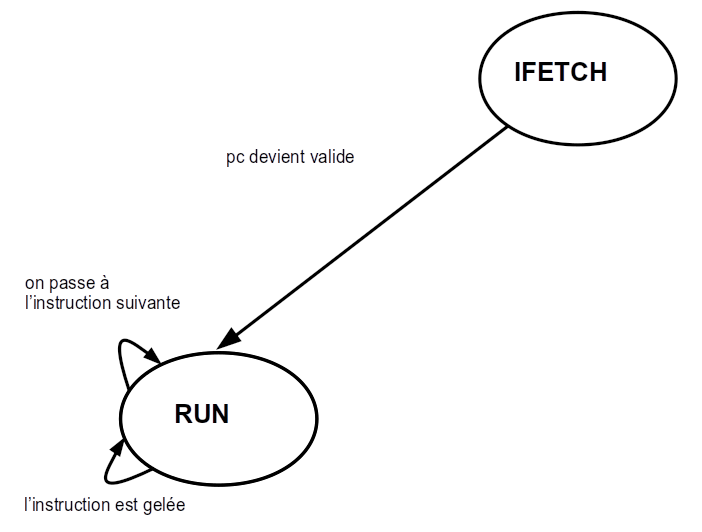
\includegraphics[width=0.75\textwidth]{pics/mae_part.png}
\centering
\caption{Un premier schema de la machine à états}
\label{mae_part}
\end{figure}


Pour l'instant ces deux états suffisent à l'implémentation des regops, mais par la suite,
nous ajouterons les états suivants :
\begin{itemize}
 \item l'état BRANCH dans lequel DECOD annulera l'execution des instruction déja chargées dans le pipeline
       et lancera le calcul du nouveau PC.

       \textit{Comme un nouveau PC est calculé, il a été invalidé donc on retourne à l'état FETCH où on attendra
       la revalidation de PC.}
 \item L'état LINK dans lequel DECOD lancera et attendra le calcul de l'adresse de retour avant de branch

       \textit{Une fois que le LINK est fait on peut brancher, donc on passera à l'état BRANCH}
 \item L'état MTRANS dans lequel DECOD restera en boucle à envoyer toutes les instructions de transfert simples
       contenues dans le transfert multiple.

       \textit{Une fois qu'on a terminé on retourne simplement à l'état normal RUN, sauf si le transfert multiple a
       modifié R15 auquel cas on passe à l'état BRANCH.}
\end{itemize}

Tous ces éléments aboutissent à la machine a états en Figure \ref{mae}.

\begin{figure}[H]
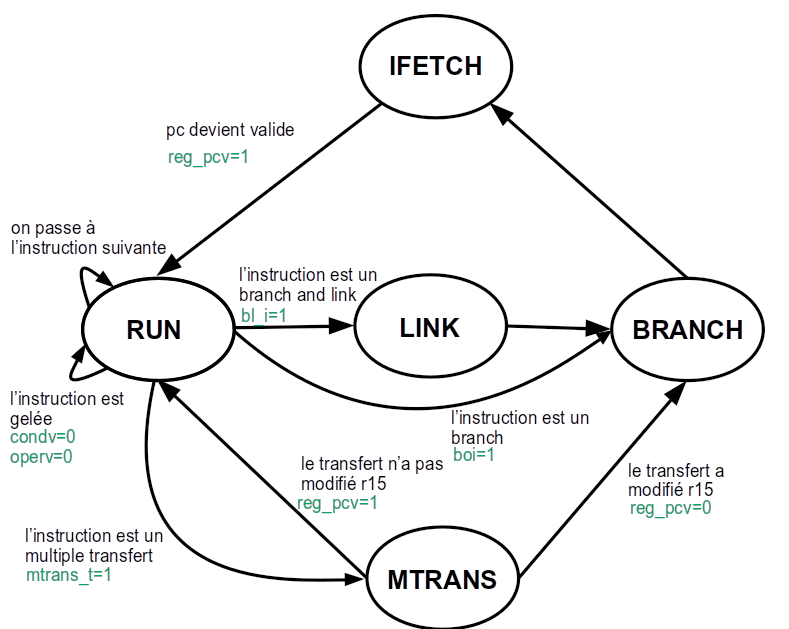
\includegraphics[width=0.75\textwidth]{pics/mae.png}
\centering
\caption{Schema final de la machine à états}
\label{mae}
\end{figure}

\subsection{Résumé de DECOD}

Tout ce que nous avons vu sur la modélisation de DECOD mène au schema en Figure \ref{dec}.

\begin{figure}[H]
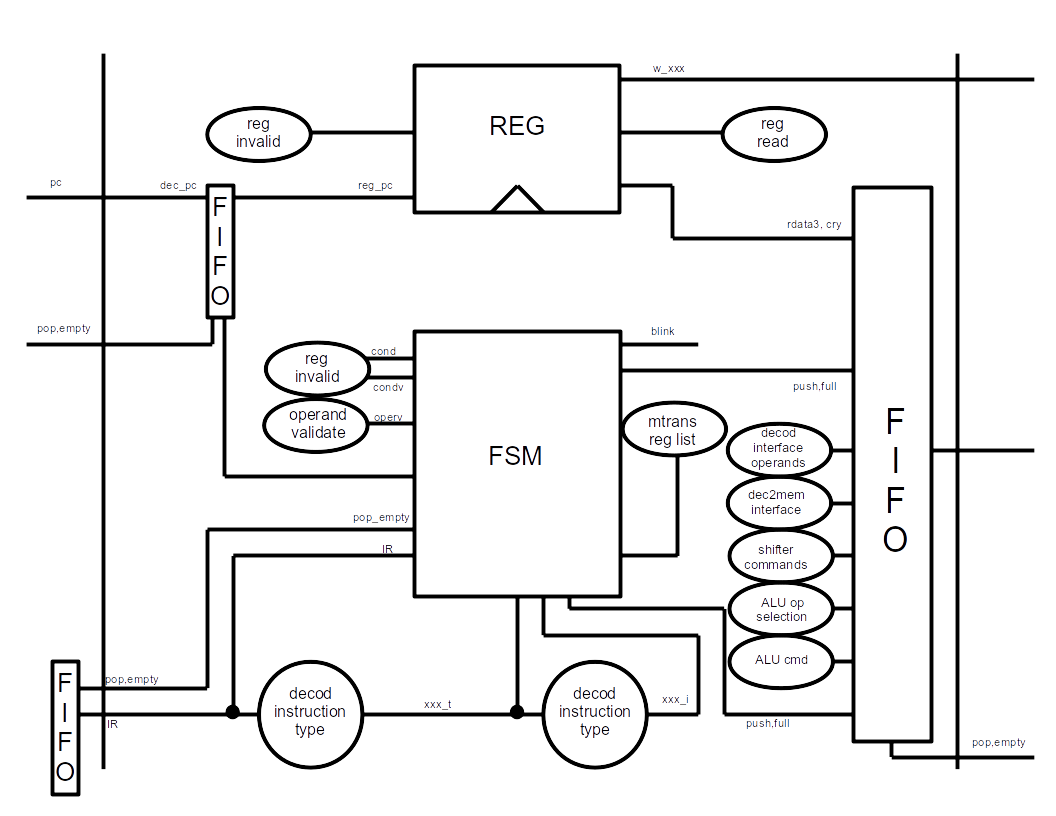
\includegraphics[width=\textwidth]{pics/dec.png}
\centering
\caption{Schema final de l'étage DECOD}
\label{dec}
\end{figure}

\section{Bilan}

Jusqu'ici, nous en sommes à l'étape de Modélisation, nous avons modélisé l'intégralité de l'étage EXE
et le socle de base de l'étage DECOD, ainsi que l'implémentation des instructions de data processing dans DECOD.
Pour remplir le cahier des charges, il nous restera à implémenter les instructions de branchements, de
transferts mémoires simples et multiples, puis il reste les étapes de Synthèse, Placement et Routage.

Une fois que cela sera implémenté, pour aboutir à un processeur capable d'exécuter un système d'exploitation
(une distribution de Linux par exemple), il restera des fonctionnalités à implémenter comme par exemple
un mécanisme de gestion de la mémoire virtuelle, des bypass ou encore la gestion d'interruption.

%==================================================================================================
%=========================  End of the Document  ==================================================
%==================================================================================================

\end{document}
